\selectlanguage{english}

\chapter{Reject Inference: a rationale review} \label{chap2}

\epigraph{Sounds good, doesn't work.}{Donald J.\ Trump}

\minitoc

%\textit{Nota Bene :} ce chapitre s'inspire fortement de l'article [...]

\bigskip

The granting process of all credit institutions is based on the probability that the applicant will refund his loan given his characteristics. This probability also called \gls{score} is learnt based on a dataset in which rejected applicants are \textit{de facto} excluded (see Section~\ref{subsec:critere}). This implies that the population on which the \gls{score} is used will be different from the learning population. Thus, this biased learning can have consequences on the scorecard's relevance. Many methods dubbed ``reject inference'' have been developed in order to try to exploit the data available from the rejected applicants to build the score. However most of these methods are considered from an empirical point of view, and there is some lack of formalization of the assumptions that are really made, and of the theoretical properties that can be expected. We propose a formalisation of these usually hidden assumptions for some of the most common reject inference methods, and we discus the improvement that can be expected. These conclusions are illustrated on simulated data and on real data from \gls{cacf}.

\section{Introduction}

In consumer loans, the acceptance process was described in Chapter~\ref{chap1} and can be formalized as follows. For a new applicant's profile and credit's characteristics, the lender aims at estimating the repayment probability. To this end, the \textit{credit modeler} fits a predictive model, often a \gls{lr}, between already  financed  clients' characteristics $\glssymbol{bx}=(\glssymbol{x}_1,\ldots,\glssymbol{x}_d)$ and their repayment status, a binary variable $\glssymbol{y}\in\{0,1\}$ (where $1$ corresponds to good clients and $0$ to bad clients). The model is then applied to the new applicant and yields an estimate of its repayment probability, called \gls{score} after an increasing transformation (see Section~\ref{subsec:apprentissage}).
%In practice, an increasing transformation of this probability also called score is often considered.
Under some cut-off value of the \gls{score}, the applicant is rejected, except if further expert rules come into play as can be seen from Figure~\ref{fig:figure1}.

\begin{figure}[ht]
\begin{minipage}[b]{0.45\linewidth}
\center \includegraphics[width=5cm]{figures/chapitre2/schema.png}
\caption{Simplified Acceptance mechanism in~Crédit Agricole Consumer Finance}
\label{fig:figure1}

\end{minipage}%
\hfil \begin{minipage}[b]{0.5\linewidth}

\center 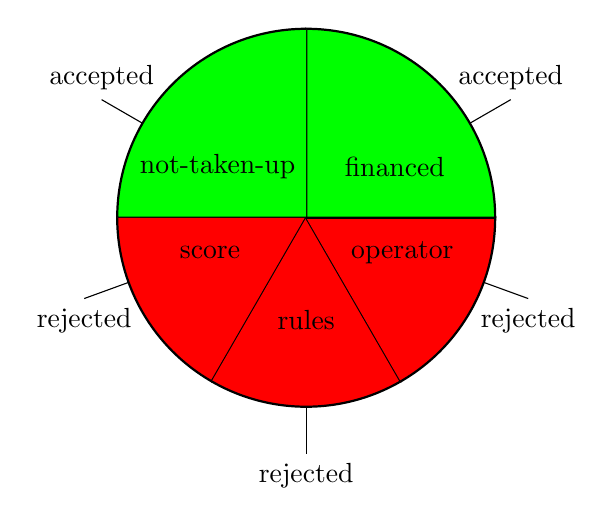
\begin{tikzpicture}

    \foreach \start/\end/\middle/\percent/\anchor/\name in {
      0/90/30/financed/above/accepted,
      90/180/150/not-taken-up/above/accepted}
  {
    \draw[fill=green, thick] (0,0) -- (\end:2.4cm) arc (\end:\start:2.4cm)
      node at (\middle:1.3cm) {\percent};
    \draw (\middle:2.4cm) -- (\middle:3cm) node[\anchor] {\name};
  };
    
    \foreach \start/\end/\middle/\percent/\anchor/\name in {
      180/240/200/score/below/rejected,
      240/300/270/rules/below/rejected,
      300/360/340/operator/below/rejected}
  {
    \draw[fill=red, thick] (0,0) -- (\end:2.4cm) arc (\end:\start:2.4cm)
      node at (\middle:1.3cm) {\percent};
    \draw (\middle:2.4cm) -- (\middle:3cm) node[\anchor] {\name};
  };
\end{tikzpicture}
\caption{Simplified Acceptance status in Crédit Agricole Consumer Finance - scale relations not respected}
\label{fig:figure2}

\end{minipage}
\end{figure}
 


The through-the-door population (all applicants) can be classified into two categories thanks to a binary variable $z$ taking values in $\{\f,\nf\}$ where $\f$ stands for financed applicants (in \textcolor{green}{green} on Figure~\ref{fig:figure2}) and $\nf$ for not financed ones (in \textcolor{red}{red} on FIgure~\ref{fig:figure2}). As the repayment variable $\glssymbol{y}$ is unobserved for not financed applicants, credit scorecards are only constructed on financed clients' data but then applied to the whole  through-the-door population. The relevance of this process is a natural question which is dealt in the field of {reject inference}. The idea is to use the characteristics of not financed clients in the scorecard building process to avoid a population bias, and thus to improve the prediction on the whole through-the-door population. Such methods have been described in~\cite{RI6,saporta,banasik,economix}, and have also notably been investigated in~\cite{RI2} who first saw {reject inference} as a missing data problem. In~\cite{RI3}, the misspecified model case on real data is studied specifically and is also developed here.


In fact, it can be considered as a part of the semi-supervised learning setting, which consists in learning from both labelled and unlabelled data. However, in the semi-supervised setting~\cite{ChaSchZie06} it is generally assumed that labelled data and unlabelled data come from the same distribution, which is rarely the case in \textit{Credit Scoring}. Moreover, the main use case of semi-supervised learning is when the number of unlabelled data is far larger than the number of labelled data, which is not the case in \textit{Credit Scoring} since the number of rejected clients and accepted clients is often balanced and depends heavily on the financial institution, the portfolio considered, etc.


The purpose of the present chapter is twofold: a clarification of which mathematical hypotheses, if any, underlie those reject inference methods and a clear conclusion on their relevance. In Section~\ref{sec:criteres}, we present a criterion to assess a method's performance and discuss missingness mechanisms that characterize the relationship of $\glssymbol{z}$ with respect to $\glssymbol{bx}$ and $\glssymbol{y}$. In Section~\ref{sec:methods_reject}, we go through some of the most common reject inference methods and exhibit their mathematical properties. 
%Finally, to confirm our theoretical findings, we test each method on simulated and real data from Crédit Agricole Consumer Finance in Section~\ref{sec:num_exp_reject}.
Finally, some guidelines are given to practitioners in Section~\ref{sec:conclusion_reject}.
%\textcolor{blue}{CB : ajouter description partie 5 (conclusion)}

\section{\textit{Credit Scoring} modelling} \label{sec:criteres}

\subsection{Data} 

The decision process of financial institutions to accept a credit application is usually embedded in the  probabilistic framework. The latter offers rigorous tools for taking into account both the variability of applicants and the uncertainty on their ability to pay back the loan. In this context, the important term is $p(\glssymbol{y}|\glssymbol{bx})$, designing the probability that a new applicant (described by his characteristics $\glssymbol{bx}$) will pay back his loan ($\glssymbol{y}=1$) or not ($\glssymbol{y}=0$). Estimation of $p(\glssymbol{y}|\glssymbol{bx})$ is thus an essential task of any \textit{Credit Scoring} process.

To perform estimation, a specific $n + m$-sample $\glssymbol{T}$ is available, decomposed into two disjoint and meaningful subsets, denoted by $\glssymbol{Tf}$ and $\glssymbol{Tnf}$ ($\glssymbol{T}=\glssymbol{Tf} \sqcup \glssymbol{Tnf} \equiv \glssymbol{T}=\glssymbol{Tf} \cup \glssymbol{Tnf}$, $\glssymbol{Tf} \cap \glssymbol{Tnf}=\emptyset$). The first subset ($\glssymbol{Tf}$) corresponds to $n$ applicants with features $\glssymbol{bx}_i$ who have been financed ($\glssymbol{z}_i={\text{f}}$) and, consequently, for who the repayment status $\glssymbol{y}_i$ is known, with their respective matrix notation $\glssymbol{bbx}_\f$, $\glssymbol{bbz}_\f$ and $\glssymbol{bby}_\f$. Thus, $\glssymbol{Tf}=(\glssymbol{bx}_i,\glssymbol{y}_i,\glssymbol{z}_i)_{i\in \text{F}} = (\glssymbol{bbx}_\f,\glssymbol{bby}_\f,\glssymbol{bbz}_\f)$ where $\text{F}=\{i:\glssymbol{z}_i={\text{f}}\}$ denotes the corresponding subset of indexes. The second subset ($\glssymbol{Tnf}$) corresponds to $m$ applicants with features $\glssymbol{bx}_i$ who have {\it not} been financed ($\glssymbol{z}_i={\text{nf}}$) and, consequently, for who the repayment status $\glssymbol{y}_i$ is {\it unknown}, with their respective matrix notation $\glssymbol{bbx}_{\text{nf}}$ and $\glssymbol{bbz}_{\text{nf}}$. Thus, $\glssymbol{Tnf}=(\glssymbol{bx}_i,\glssymbol{z}_i)_{i\in \text{NF}} = (\glssymbol{bbx}_{\text{nf}}, \glssymbol{bbz}_{\text{nf}})$ where $\text{NF}=\{i:z_i={\text{nf}}\}$ denotes the corresponding subset of indexes. We notice that $\glssymbol{y}_i$ values are excluded from the observed sample $\glssymbol{Tnf}$, since they are missing. These data can be represented schematically as:

\[ \glssymbol{T} = \begin{array}{c}
\glssymbol{Tf} = \bigg( \; \tikzmarkin[hor=style green]{el02} \glssymbol{bbx}_{\text{f}} \tikzmarkend{el02}\\
\\
\sqcup \\
\\
\glssymbol{Tnf} = \bigg( \; \tikzmarkin[hor=style orange]{el-12} \glssymbol{bbx}_{\text{nf}} \tikzmarkend{el-12} \end{array}
\left( \begin{array}{ccc}
%\rowcolor{red!20}
\tikzmarkin[hor=style green]{e1} \; \; x_1^1 & \cdots & x_1^d  \\
 \vdots & \vdots & \vdots  \\
 x_n^1 & \cdots & x_n^d \tikzmarkend{e1} \\
\tikzmarkin[hor=style orange]{e2} \; \; x_{n+1}^1 & \cdots & x_{n+1}^d  \\
 \vdots & \vdots & \vdots \\
 x_{n+m}^1 & \cdots & x_{n+m}^d \tikzmarkend{e2} \end{array} \right),
 \hspace{1.5cm}
 \begin{array}{c}
\tikzmarkin[hor=style green]{el11} \glssymbol{bby}_{\text{f}} \tikzmarkend{el11}\\
\\
\\
\\
\tikzmarkin[hor=style orange]{el12} \glssymbol{bby}_{\text{nf}} \tikzmarkend{el12}\end{array}
\left( \begin{array}{c}
\tikzmarkin[hor=style green]{e4} y_1 \\
\vdots \\
y_n \tikzmarkend{e4} \\ 
\tikzmarkin[hor=style orange]{e3} \text{NA} \\
\vdots \\
\text{NA} \tikzmarkend{e3} \end{array} \right) ,
 \hspace{1.5cm}
 \begin{array}{c}
\tikzmarkin[hor=style green]{el111} \glssymbol{bbz}_{\text{f}} \tikzmarkend{el111}\\
\\
\\
\\
\tikzmarkin[hor=style orange]{el121} \glssymbol{bbz}_{\text{nf}} \tikzmarkend{el121}\end{array}
\left( \begin{array}{c}
\tikzmarkin[hor=style green]{e41} \text{f} \\
\vdots \\
\text{f} \tikzmarkend{e41} \\ 
\tikzmarkin[hor=style orange]{e31} \text{nf} \\
\vdots \\
\text{nf} \tikzmarkend{e31} \end{array} \right)
 \hspace{0.2cm}
 \begin{array}{c}
\bigg). \\
\\
\\
\\
\bigg). \end{array}
\]


\subsection{General parametric model}

Estimation of $p(\glssymbol{y}|\glssymbol{bx})$ has to rely on modelling since the true probability distribution is unknown. Firstly, it is both convenient and realistic to assume that triplets $(\glssymbol{bx}_i,\glssymbol{y}_i,\glssymbol{z}_i)_{1\le i\le n}$ are all independent and identically distributed (i.i.d.), including the unknown values of $\glssymbol{y}_i$ when $i\in \text{NF}$. Secondly, it is usual and convenient to assume that the unknown distribution $p(\glssymbol{y}|\glssymbol{bx})$ belongs to a given parametric family $\{p_{\glssymbol{bth}}(\glssymbol{y}|\glssymbol{bx})\}_{\glssymbol{bth} \in\Theta}$, where $\Theta$ is the parameter space as was discussed in Chapter~\ref{chap1}. For instance, \gls{lr} is often considered in practice, even if we will be more general in this section. However, \gls{lr} will be important for other sections since some standard reject inference methods are specific to this family (Section~\ref{sec:methods_reject}) and numerical experiments (Section~\ref{sec:experiments_reject}) will implement them.

As in any missing data situation (here $\glssymbol{z}$ indicates if $\glssymbol{y}$ is observed or not), the relative modelling process, namely $p(\glssymbol{z}|\glssymbol{bx},\glssymbol{y})$, has also to be clarified. For convenience, we can also consider a parametric family $\{p_{\glssymbol{phi}}(\glssymbol{z}|\glssymbol{bx},\glssymbol{y})\}_{\glssymbol{phi} \in \Phi}$, where $\glssymbol{phi}$ denotes the parameter and $\Phi$ the associated parameter space of the financing mechanism. Note we consider here the most general missing data situation, namely a \glsfirst{mnar} mechanism~\cite{littlerubin}. It means that $\glssymbol{z}$ can be stochastically dependent on some missing data $\glssymbol{y}$, namely that $p(\glssymbol{z}|\glssymbol{bx},\glssymbol{y})\neq p(\glssymbol{z}|\glssymbol{bx})$. We will discuss this fact in Section~\ref{sec:mechanisms}.

Finally, combining both previous distributions $p_{\glssymbol{bth}}(\glssymbol{y}|\glssymbol{bx})$ and $p_{\glssymbol{phi}}(\glssymbol{z}|\glssymbol{bx},\glssymbol{y})$ leads to express the joint distribution of $(\glssymbol{y},\glssymbol{z})$ conditionally to $\glssymbol{bx}$ as:
\begin{equation}\label{eq:generative}
p_{\gamma}(\glssymbol{y},\glssymbol{z}|\glssymbol{bx}) = p_{\glssymbol{phi}(\gamma)}(\glssymbol{z}|\glssymbol{y},\glssymbol{bx})p_{\glssymbol{bth}(\gamma)}(\glssymbol{y}|\glssymbol{bx}).
\end{equation}
where $\{p_{\gamma}(\glssymbol{y},\glssymbol{z}|\glssymbol{bx})\}_{\gamma \in \Gamma}$ denotes a distribution family indexed by a parameter $\gamma$ evolving in a space $\Gamma$. Here it is clearly expressed that both parameters $\glssymbol{phi}$ and $\glssymbol{bth}$ can depend on $\gamma$, even if in the following we will note shortly $\glssymbol{phi}=\glssymbol{phi}(\gamma)$ and $\glssymbol{bth}=\glssymbol{bth}(\gamma)$. In this very general missing data situation, the missing process is said to be {\it non-ignorable}, meaning that parameters $\glssymbol{phi}$ and $\glssymbol{bth}$ can be functionality dependent (thus $\gamma\neq (\glssymbol{phi},\glssymbol{bth})$). We also discuss this fact in Section~\ref{sec:mechanisms}.

\subsection{Maximum likelihood estimation} 
\label{sec:EM}

Mixing previous model and data, the maximum likelihood principle can be invoked for estimating the whole parameter $\gamma$, thus yielding as a by-product an estimate of the parameter $\glssymbol{bth}$. Indeed, $\glssymbol{bth}$ is of particular interest, the goal of the financial institutions being solely to obtain an estimate of $p_{\glssymbol{bth}}(\glssymbol{y}|\glssymbol{bx})$. The observed log-likelihood can be written as:
\begin{equation}\label{eq:like.MNAR}
\ell(\gamma;\glssymbol{T}) = \sum_{i\in\text{F}}\ln p_{\gamma}(\glssymbol{y}_i,\text{f} | \glssymbol{bx}_i) + \sum_{i'\in\text{NF}} \ln \left[ \sum_{\glssymbol{y}\in\{0,1\}} p_{\gamma}(\glssymbol{y},\text{nf} | \glssymbol{bx}_{i'}) \right].
\end{equation}
Within this missing data paradigm, the EM algorithm (see~\cite{dempster1977maximum}) can be used. Starting from an initial value $\gamma^{(0)}$, iteration $(s)$ of the algorithm is decomposed into the following two classical steps:
\paragraph{E-step} compute the conditional probabilities of missing $\glssymbol{y}_i$ values:
\begin{equation}
t_{i\glssymbol{y}}^{(s)} = p_{\glssymbol{bth}(\gamma^{(s-1)})}(\glssymbol{y}|\glssymbol{bx}_i,\nf) = \frac{p_{\gamma^{(s-1)}}(\glssymbol{y}, \nf|\glssymbol{bx}_i)}{\sum_{\glssymbol{y}' = 0}^{1} p_{\gamma^{(s-1)}}(\glssymbol{y}', \nf|\glssymbol{bx}_i)};
\end{equation}
\paragraph{M-step} maximize the conditional expectation of the complete log-likelihood:
\begin{equation}\label{eq:like.c}
\ell_c(\gamma;\glssymbol{T}_c) = \sum_{i=1}^{n+m}\ln p_{\gamma}(\glssymbol{y}_i,\glssymbol{z}_i | \glssymbol{bx}_i);
\end{equation}
leading to:
\begin{equation}
\gamma^{(s)} = \argmax_{\gamma \in \Gamma} \sum_{i\in \text{F}} \ln p_{\gamma}(\glssymbol{y}_i, \f|\glssymbol{bx}_i) +  \sum_{i'\in \text{NF}}\sum_{\glssymbol{y} = 0}^{1}t_{i'\glssymbol{y}}^{(s)} \ln p_{\gamma}(\glssymbol{y}, \nf | \glssymbol{bx}_{i'}).
\end{equation}
Usually, stopping rules rely either on a predefined number of iterations, or on a predefined stability criterion of the observed log-likelihood.

\subsection{Some current restrictive missingness mechanisms}
\label{sec:mechanisms}

The latter parametric family is very general since it considers both that the missingness mechanism is \gls{mnar} and non-ignorable. But in practice, it is common to consider ignorable models for the sake of simplicity, meaning that $\gamma= (\glssymbol{phi},\glssymbol{bth})$. There exists also some restrictions to the \gls{mnar} mechanism. 

The first restriction to \gls{mnar} is the \glsfirst{mcar} setting, meaning that $p(\glssymbol{z}| \glssymbol{bx},\glssymbol{y}) = p(\glssymbol{z})$. In that case, applicants should be accepted or rejected without taking into account their descriptors $\glssymbol{bx}$. Such a process is not realistic at all for representing the actual process followed by financial institutions. Consequently it is always discarded in \textit{Credit Scoring}.

The second restriction to \gls{mnar} is the \glsfirst{mar} setting, meaning that $p(\glssymbol{z}| \glssymbol{bx},\glssymbol{y}) = p(\glssymbol{z}|\glssymbol{bx})$. The \gls{mar} missingness mechanism seems realistic for \textit{Credit Scoring} applications, for example when financing is based solely on a function of $\glssymbol{bx}$, {\it e.g.} in the case of a score associated to a cut-off, provided all clients' characteristics of this existing \gls{score} are included in $\glssymbol{bx}$. It is a usual assumption in \textit{Credit Scoring} even if, in practice, the financing mechanism may depend also on unobserved features (thus not present in $\glssymbol{bx}$), which is particularly true when an operator (see Figure~\ref{fig:figure1}) adds a subjective, often intangible, expertise. In the \gls{mar} situation the log-likelihood~(\ref{eq:like.MNAR}) can be reduced to:
\begin{equation}\label{eq:like.MAR}
\ell(\gamma;\glssymbol{T}) = \ell(\glssymbol{bth};\glssymbol{Tf}) + \sum_{i'=1}^n \ln p_{\glssymbol{phi}}(\glssymbol{z}_{i'} | \glssymbol{bx}_{i'}),
\end{equation}
with $\ell(\glssymbol{bth};\glssymbol{Tf})=\sum_{i\in\text{F}}\ln p_{\glssymbol{bth}}(\glssymbol{y}_i | \glssymbol{bx}_i)$.
Combining it with the ignorable assumption, estimation of $\glssymbol{bth}$ relies only on the first part $\ell(\glssymbol{bth};\glssymbol{Tf})$, since the value $\glssymbol{phi}$ has no influence on~$\glssymbol{bth}$. In that case, invoking an EM algorithm due to missing data $\glssymbol{y}$ is no longer required as will be made explicit in Section~\ref{subsec:strat1}.

\subsection{Model selection} \label{subsec:model_selection}

At this step, several kinds of parametric model~(\ref{eq:generative}) have been assumed. It concerns obviously the parametric family $\{p_{\glssymbol{bth}}(\glssymbol{y}|\glssymbol{bx})\}_{\glssymbol{bth} \in\Theta}$, and also the missingness mechanism \gls{mar} or \gls{mnar}. 
However, it has to be noticed that \gls{mar} versus \gls{mnar} cannot be tested since we do not have access to $\glssymbol{y}$ for not financed clients~\cite{molenberghs2008every}. However, model selection is possible by modelling also the whole financing mechanism, namely the family $\{p_{\glssymbol{phi}}(\glssymbol{z}|\glssymbol{bx},\glssymbol{y})\}_{\glssymbol{phi} \in \Phi}$.


Scoring for credit application can be recast as a semi-supervised classification problem~\cite{Chapelle:2010:SL:1841234}. In this case, classical model selection criteria can be divided into two categories~\cite{vandewalle:tel-00447141}: either scoring performance criteria as \textit{e.g.}\ error rate on a test set $\glssymbol{T}^{\text{test}}$, or information criteria like \textit{e.g.}\ BIC as was introduced in Section~\ref{subsubsec:choix_modele}.

In the category of error rate criteria, the typical error rate is expressed as follows:
\begin{equation} \label{eq:error}
\mbox{Error}(\glssymbol{T}^\text{test}) = \frac{1}{|\glssymbol{T}^\text{test}|} \sum_{y_i \in \glssymbol{T}^\text{test}} \mathbb{I}(\hat y_i \neq y_i),
\end{equation} 
where $\glssymbol{T}^\text{test}$ is a an i.i.d. test sample from $p(\glssymbol{y}|\glssymbol{bx})$ and where $\hat{\glssymbol{y}}_i$ is the estimated value of the related $\glssymbol{y}_i$ value involved by the estimated model at hand. The model leading to the lowest error value is then retained. However, in the \textit{Credit Scoring} context this criterion family is not available since no sample $\glssymbol{T}^\text{test}$ is itself available. This problem can be exhibited through the following straightforward expression
\begin{equation} \label{eq:error2}
p(\glssymbol{y}|\glssymbol{bx}) = \sum_{\glssymbol{z}\in\{\text{f},\text{nf}\}} p(\glssymbol{y}|\glssymbol{bx},\glssymbol{z}) p(\glssymbol{z}|\glssymbol{bx})
\end{equation}
where $p(\glssymbol{y}|\glssymbol{bx},\glssymbol{z})$ is unknown and $p(\glssymbol{z}|\glssymbol{bx})$ is known since this latter is defined by the financial institution itself. We notice that obtaining a sample from $p(\glssymbol{y}|\glssymbol{bx})$ would require that the financial institution draws $\glssymbol{bbz}^\text{test}$ i.i.d. from $p(\glssymbol{z}|\glssymbol{bx})$ before to observe the results $\glssymbol{bby}^\text{test}$ i.i.d. from $p(\glssymbol{y}|\glssymbol{bx},\glssymbol{z})$. But in practice it is obviously not the case, a threshold being applied to the distribution $p(\glssymbol{z}|\glssymbol{bx})$ for retaining only a set of fundable applicants, the non-fundable applicants being definitively discarded, preventing us from getting a test sample $\glssymbol{T}^\text{test}$ from $p(\glssymbol{y} | \glssymbol{bx})$. As a matter of fact, only a sample $\glssymbol{T}^\text{test}_{\text{f}}$ of $p(\glssymbol{y}|\glssymbol{bx},\text{f})$ is available, 
irrevocably prohibiting the calculus of~(\ref{eq:error}) as a model selection criterion.

In the category of information criteria, the BIC criterion (presented in Section~\ref{subsubsec:choix_modele}) is expressed as the following penalization of the maximum log-likelihood:
\begin{equation}\label{eq:AIC}
\mbox{BIC} = - 2 \ell(\hat\gamma;\glssymbol{T}) + dim(\Gamma) \ln n,
\end{equation}
where $\hat\gamma$ is the maximum likelihood estimate of $\gamma$ and $dim(\Gamma)$ is the number of parameters to be estimated in the model at hand. The model leading to the lowest BIC value is then retained. Many other BIC-like criteria exist~\cite{vandewalle:tel-00447141} but the underlined idea is unchanged. Contrary to the error rate criteria like~(\ref{eq:error}), it is thus possible to compare models without funding ``non-fundable applicants'' since just the available sample $\glssymbol{T}$ is required. However, computing~(\ref{eq:AIC}) requires to precisely express the model families $\{p_{\gamma}(\glssymbol{y},\glssymbol{z}|\glssymbol{bx})\}_{\gamma \in \Gamma}$ which compete.

\section{Rational reinterpretation of \textit{reject inference} methods} \label{sec:methods_reject}

\subsection{The reject inference challenge} \label{subsec:challenge}

As discussed in the previous section, a regular way to use the whole observed sample $\glssymbol{T}$ in the estimation process implies some challenging modelling and assumption steps. A method using the whole sample $\glssymbol{T}$ is traditionally called a {\it rejection inference} method since it uses not only financed applicants (sample $\glssymbol{Tf}$) but also not financed, or rejected, applicants (sample $\glssymbol{Tnf}$).
Since modelling the financing mechanism $p(\glssymbol{z} | \glssymbol{bx}, \glssymbol{y})$ is sometimes a too heavy task, such methods propose alternatively to use the whole sample $\glssymbol{T}$ in a more empirical manner. However, this is somehow a risky strategy since we have also seen in the previous section that validating methods with error rate like criteria is not possible through the standard \textit{Credit Scoring} process. As a result, some strategies are proposed to perform a ``good'' \gls{score} function estimation without possibility to access their real performance.

However, most of the proposed reject inference strategies may make some hidden assumptions on the modelling process. Our challenge is to reveal as far as possible such hidden assumptions to then discuss their realism,  
failing to be able to compare them by the model selection principle.

\subsection{Strategy 1: ignoring not financed clients} \label{subsec:strat1}

\subsubsection{Definition}
The simplest reject inference strategy is to ignore not financed clients for estimating $\glssymbol{bth}$. Thus it consists to estimate $\glssymbol{bth}$ by maximizing the log-likelihood $\ell(\glssymbol{bth};\glssymbol{Tf})$.

\subsubsection{Interpretation}
In fact, this strategy is equivalent to using the whole sample $\glssymbol{T}$ (financed and not financed applicants) under both the \gls{mar} and ignorable assumptions. See the related explanation in Section~\ref{sec:mechanisms}. Consequently, this strategy is truly a particular ``reject inference'' strategy although it does not seem to be.

\subsubsection{In details}
By denoting by $\hat{\glssymbol{bth}}_\text{f}$ and $\hat{\glssymbol{bth}}$ respectively the maximum likelihood estimates of $\ell(\glssymbol{bth};\glssymbol{Tf})$ and $\ell(\glssymbol{bth};\glssymbol{T})$ provided we know $\glssymbol{y}_i$ for $i \in \text{NF}$, classic maximum likelihood properties~\cite{10.2307/1912526,zadrozny2004learning} yield under a well-specified model hypothesis (there exists $\glssymbol{bthstar}$ s.t.\ $p(\glssymbol{y} | \glssymbol{bx}) = p_{\glssymbol{bthstar}}(\glssymbol{y} | \glssymbol{bx})$ for all $(\glssymbol{bx},\glssymbol{y})$) and a \gls{mar} missingness mechanism that $\hat{\glssymbol{bth}} \approx \hat{\glssymbol{bth}}^\text{f}$ for large-enough samples $\glssymbol{Tf}$ and $\glssymbol{Tnf}$.



\subsection{Strategy 2: fuzzy augmentation}

\subsubsection{Definition}
This strategy corresponds to an algorithm which is starting with $\hat{\glssymbol{bth}}^{(0)} = \hat{\glssymbol{bth}}_\text{f}$ (see previous section). Then, all $(\glssymbol{y}_i)^{(1)}_{i \in \text{NF}}$ are imputed by their expected value given by: $\hat{\glssymbol{y}}^{(1)}_i = p_{\hat{\glssymbol{bth}}^{(0)}}(1 | \glssymbol{bx}_i)$ (notice that these imputed values are not in $\{0,1\}$ but in $]0,1[$). The completed log-likelihood $\ell_c(\glssymbol{bth};\glssymbol{T}_c^{(1)})$ given in~(\ref{eq:like.c}) with $\glssymbol{T}_c^{(1)}=\glssymbol{Tf} \cup (\glssymbol{y}_i)^{(1)}_{i \in \nf}$ is maximized and yields parameter estimate $\hat{\glssymbol{bth}}^{(1)}$.

\subsubsection{Interpretation}
There are two possible interpretations of this method's optimized criterion, as found in~\cite{economix}: first as a completed log-likelihood as underlined in the previous paragraph; second as a generative log-likelihood $\mathbb{E}_{\glssymbol{bby}^{\text{nf}}}\left[\ell(\glssymbol{bth};\glssymbol{bbx},\glssymbol{bby}^{\text{f}},{\glssymbol{bby}}^{\text{nf}}) \middle| \hat{\glssymbol{bth}}^{\text{f}}\right] = \ell(\glssymbol{bth};\glssymbol{bbx}^{\text{f}},\glssymbol{bby}^{\text{f}}) + \sum_{i=n+1}^{n+m} \sum_{\glssymbol{y}_i=0}^{1} \mathbb{E}\left[\glssymbol{y}_i \middle| \glssymbol{bx}_i,\hat{\glssymbol{bth}}^{\text{f}}\right] p_{\glssymbol{bth}}(\glssymbol{y}_i|\glssymbol{bx}_i)$. In a way, it is a one-step \gls{em}-algorithm, as presented in Section~\ref{sec:EM}, without taking into account the financing mechanism $p(\glssymbol{z} | \glssymbol{bx},\glssymbol{y})$.

\subsubsection{In details}
It can be easily shown (Appendix~\ref{fuzzy}) that $\argmax_{\glssymbol{bth}} \ell_c(\glssymbol{bth};\glssymbol{T}_c^{(1)}) = \hat{\theta}^{\text{f}}$ so that this method is similar to the scorecard learnt on the financed clients.

\subsection{Strategy 3: reclassification}

\subsubsection{Definition}
This strategy corresponds to an algorithm which is starting with $\hat{\glssymbol{bth}}^{(0)} = \hat{\glssymbol{bth}}_\text{f}$ (see Section~\ref{subsec:strat1}). Then, all $(\glssymbol{y}_i)^{(1)}_{i \in \text{NF}}$ are imputed by the {\it maximum a posteriori} (MAP) principle given by: $\hat{\glssymbol{y}}^{(1)}_i = \argmax_{\glssymbol{y} \in \{0,1\}} p_{\hat{\glssymbol{bth}}^{(0)}}(\glssymbol{y} | \glssymbol{bx}_i)$. The completed log-likelihood $\ell_c(\glssymbol{bth};\glssymbol{T}_c^{(1)})$ given in~(\ref{eq:like.c}) with $\glssymbol{T}_c^{(1)}=\glssymbol{Tf} \cup (\glssymbol{y}_i)^{(1)}_{i \in \nf}$ is maximized and yields parameter estimate $\hat{\glssymbol{bth}}^{(1)}$, as can be expressed schematically as:
\[ \glssymbol{T}_c^{(1)} = \begin{array}{c}
\tikzmarkin[hor=style green]{el0} \bm{x}^{\text{f}} \tikzmarkend{el0} \\
\\
\\
\tikzmarkin[hor=style green]{el-1} \bm{x}^{\text{nf}} \tikzmarkend{el-1} \end{array}
\left( \begin{array}{ccc}
%\rowcolor{red!20}
\tikzmarkin[hor=style green]{el1} \; \; x_1^1 & \cdots & x_1^d  \\
 \vdots & \vdots & \vdots \\
 x_n^1 & \cdots & x_n^d \\
 x_{n+1}^1 & \cdots & x_{n+1}^d  \\
 \vdots & \vdots & \vdots \\
 x_{n+m}^1 & \cdots & x_{n+m}^d \tikzmarkend{el1} \end{array} \right)
 \begin{array}{c}
\tikzmarkin[hor=style green]{l1} \bm{y}^{\text{f}} \tikzmarkend{l1}\\
\\
\\
\tikzmarkin[hor=style green]{l2} \bm{y}^{\text{nf}} \tikzmarkend{l2} \end{array}
\left( \begin{array}{c}
\tikzmarkin[hor=style green]{l3} \; \; y_1 \; \; \; \\
\vdots \\
 y_n \\ 
 \hat{\glssymbol{y}}_{n+1}^{(1)} \\
\vdots \\
\hat{\glssymbol{y}}_{n+m}^{(1)} \tikzmarkend{l3}\end{array} \right).\]

Its first variant stops at this value $\hat{\glssymbol{bth}}^{(1)}$. Its second variant iterates until potential convergence of $(\hat{\glssymbol{bth}}^{(s)})$, $s$ designing the iteration number. In practice, this method can be found in~\cite{saporta} under the name ``iterative reclassification'' in~\cite{RI6}, under the name ``reclassification'' or under the name ``extrapolation'' in~\cite{banasik}.

\subsubsection{Interpretation}
This algorithm is equivalent to the so-called \gls{cem} algorithm where a Classification (or MAP) step is inserted between the Expectation and Maximization steps of an \gls{em} algorithm (described in Section~\ref{sec:EM}). It can be found in \cite{RI6}, also sometimes referred to as extrapolation as in \cite{banasik}. \gls{cem} aims at maximizing the completed log-likelihood $\ell_c(\glssymbol{bth};\glssymbol{T}_c)$ over both $\glssymbol{bth}$ and $(\glssymbol{y}_i)_{i \in \nf}$. Since $\glssymbol{phi}$ is not involved in this process, we first deduce from Section~\ref{sec:mechanisms} that, again, \gls{mar} and ignorable assumptions are present. Then, standard properties of the estimate maximizing the completed likelihood indicate that it is not a consistent estimate of $\glssymbol{bth}$~\cite{celeux1992classification}, contrary to the traditional maximum likelihood one.

\subsubsection{In details}
The \gls{cem} algorithm is known for ``sharpening'' the decision boundary: predicted probabilities are closer to $0$ and $1$ than their true values as can be seen from simulated data from a \gls{mar} mechanism on Figure~\ref{fig:biais_CEM}. The scorecard $\hat{\glssymbol{bth}}_{\text{f}}$ on financed clients (in \textcolor{green}{green}) is asymptotically consistent as was emphasized in the previous section while the reclassified scorecard (in \textcolor{red}{red}) is biased. The algorithm is detailed in Appendix~\ref{reclassification}.

\begin{figure}[ht]
\center \includegraphics[width=\textwidth]{figures/chapitre2/CEM_bias.png}
\caption{In the context of a probabilistic classifier, it is known that the CEM algorithm employed implicitly by the Reclassification method amounts to a bigger bias in terms of \gls{lr} parameters, but a ``sharper'' decision boundary.}
\label{fig:biais_CEM}
\end{figure}


\subsection{Strategy 4: augmentation} \label{subsec:augmentation}

\subsubsection{Definition}
This technique is directly influenced by the Importance Sampling~\cite{zadrozny2004learning} literature because intuitively, as for all selection mechanism such as survey respondents, observations have to be weighted according to their probability of being in the sample w.r.t.\ the whole population, i.e.\ by $p(\glssymbol{z} | \glssymbol{bx},\glssymbol{y})$. By assuming implicitly a \gls{mar} missingness mechanism, as emphasized in Section~\ref{sec:mechanisms}, we get $p(\glssymbol{z} | \glssymbol{bx}; \glssymbol{y}) = p(\glssymbol{z} | \glssymbol{bx})$. However, as was also emphasized in Section~\ref{subsec:challenge}, this \gls{pdf} also has to be estimated. This method proposes to bin observations in $\glssymbol{T}$ in, say, 10 \textit{equal-length} intervals of the \gls{score} given by $p_{\hat{\glssymbol{bth}}_\text{f}}(1 | \glssymbol{bx})$ and estimate $p(\glssymbol{z} | \glssymbol{bx})$ as the proportion of financed clients in each of these bins. The inverse of this estimate is then used to weight financed clients in $\glssymbol{Tf}$ and retrain the model.

\subsubsection{Interpretation}
The methods aims at correcting for the selection procedure yielding the training data $\glssymbol{Tf}$ in the \gls{mar} case. As was argued in Section~\ref{subsec:strat1}, if the model is well-specified, such a procedure is superfluous as the estimated parameter $\hat{\glssymbol{bth}}_{\f}$ is consistent. In the misspecified case however, it is theoretically justified as will be developed in the next paragraph. However, it is unclear if this apparent benefit is not offset by the added estimation procedure (which comes with its bias / variance trade-off).

\subsubsection{In details}
In Section~\ref{subsec:gradient}, we derived the likelihood from the $\glssymbol{KL}$ divergence by focusing on $\mathbb{E}_{\glssymbol{bX},\glssymbol{Y}} [\ln[p_{\glssymbol{bth}}(\glssymbol{y}|\glssymbol{bx})]]$. By remarking that $p(\glssymbol{bx}) = \dfrac{p(\glssymbol{bx} | \f)}{p(\f | \glssymbol{bx})} p(\f) $ and by assuming a \gls{mar} missingness mechanism, we get:
\[\mathbb{E}_{\glssymbol{bX},\glssymbol{Y}} [\ln[p_{\glssymbol{bth}}(\glssymbol{y}|\glssymbol{bx})]] = p(\f) \sum_{\glssymbol{y}=0}^1 \int_{\mathcal{X}} \dfrac{\ln p_{\glssymbol{bth}}(\glssymbol{y} | \glssymbol{bx})}{p(\f | \glssymbol{bx})} p(\glssymbol{y} | \glssymbol{bx}) p(\glssymbol{bx} | \f) d\glssymbol{bx} \approx_{n \to \infty} \dfrac{p(\f)}{n} \sum_{i=1}^n \dfrac{1}{p(\f | \glssymbol{bx}_i)} \ln p_{\glssymbol{bth}}(\glssymbol{y}_i | \glssymbol{bx}_i).\]
Consequently, had we access to $p(\f | \glssymbol{bx})$, the parameter maximizing the above mentioned likelihood would asymptotically be equal to the one on the through-the-door population, had we access to $\glssymbol{bby}^\nf$. However, $p(\f | \glssymbol{bx})$ can be estimated by the practitioner's method of choice, which will come with its bias and variance. Additionally, the Importance Sampling paradigm requires $p(\f | \glssymbol{bx}) > 0$ for all $\glssymbol{bx}$ which is clearly not the case here: for example, jobless people are never financed.

\subsection{Strategy 5: twins}

\subsubsection{Definition}
This \textit{Reject Inference} method is documented internally at \gls{cacf} and in Appendix~\ref{Twins}; it consists in combining two scorecards: one predicting $\glssymbol{y}$ learnt on financed clients (denoted by $\hat{\glssymbol{bth}}_{\text{f}}$ as previously), the other predicting $\glssymbol{z}$ learnt on all applicants, before learning the final scorecard using the predictions made by both scorecards on financed clients.

\subsubsection{Interpretation}
The method aims at re-injecting information about the financing mechanism in the \gls{mar} missingness mechanism by estimating $\hat{\glssymbol{phi}}$ as a \gls{lr} on all applicants, calculating \gls{score}s $(1,\glssymbol{bx})' \hat{\glssymbol{bth}}_\f$ and $(1,\glssymbol{bx})' \hat{\glssymbol{phi}}$ and use these as two continuous features in a third \gls{lr} predicting again the repayment feature $\glssymbol{y}$.

\subsubsection{In details}
It can be easily shown (Appendix~\ref{Twins}) that $\argmax_{\glssymbol{bth}} \ell(\glssymbol{bth};(\bm{1},\glssymbol{bbx})' \hat{\glssymbol{phi}}, (\bm{1},\glssymbol{bbx})' \hat{\glssymbol{bth}}_\f, \glssymbol{bby}) = \hat{\theta}^{\text{f}}$ so that this method is similar to the scorecard learnt on the financed clients.

\subsection{Strategy 6: parcelling} \label{subsec:parcel}

\subsubsection{Definition}
The Parcelling method can be found in~\cite{saporta,banasik,RI6}. It is also described in Appendix~\ref{Parceling}. This method aims to correct the log-likelihood estimation in the \gls{mnar} case by making further assumptions on $p(\glssymbol{y} | \glssymbol{bx}, \glssymbol{z})$. It is a little deviation from the fuzzy augmentation method in a \gls{mnar} setting: we start with $\hat{\glssymbol{bth}}^{(0)} = \hat{\glssymbol{bth}}_\f$ and then impute $(\glssymbol{y}_i)_{i \in \text{NF}}^{(1)}$ by a user-defined prudence factor over their expected value (see next paragraphs).

\subsubsection{Interpretation}
By considering not-financed clients as riskier than financed clients with the same level of \gls{score}, \textit{i.e.}\ $p(\glssymbol{y} | \glssymbol{bx}, \nf) > p(\glssymbol{y} | \glssymbol{bx}, \f)$, it is implicitly assumed that manual operators (see Figure~\ref{fig:figure1}) have access to additional information, say $\tilde{\glssymbol{bx}}$, that influence the outcome $\glssymbol{y}$ even when $\glssymbol{bx}$ is accounted for, such that rejected and accepted clients with the same \gls{score} defer only by $\tilde{\glssymbol{bx}}$, which we do not have access to and is accounted for in a user-defined prudence factor stating that rejected clients would have been riskier than accepted ones.

\subsubsection{In details}
A completed dataset $\glssymbol{T}_c$ is derived by making bins of observations in $\glssymbol{T}$ in, say, 10 \textit{equal-length} intervals of the \gls{score} given by $p_{\hat{\glssymbol{bth}}_\text{f}}(1 | \glssymbol{bx})$ and estimate $p(\glssymbol{y} | \glssymbol{bx}, \nf)$ as the mean of $\glssymbol{Y} | \glssymbol{bx}, \f$ in each bin multiplied by a prudence factor encompassing the practitioner's \textit{belief} about the effectiveness of the operators' rejections.

\bigskip

Since it is possible to conclude about these reject inference methods analytically (see next section), simulations and numerical experiments on real data have been deferred to the Appendices~\ref{subsec:app_reject_sim}, \ref{subsec:app_reject_real} and~\ref{subsec:app_reject_real_method} where reject inference methods are applide on simulated data and real data and compared to other predictive methods respectively.

%\section{Numerical experiments} \label{sec:num_exp_reject}

\section{Discussion: choosing the right model} \label{sec:conclusion_reject}

\subsection{Sticking with the financed clients model}

Constructing scorecards by using a \gls{lr} on financed clients is a trade-off: on the one hand, it is implicitly assumed that it is well-specified, and that the missingness mechanism governing the observation of $\glssymbol{Y}$ is \gls{mar}. In other words, we suppose $p(\glssymbol{y} | \glssymbol{bx}) = p_{\glssymbol{bthstar}}(\glssymbol{y} | \glssymbol{bx}, \f)$. On the other hand, these assumptions, which seem strong at first hand, cannot really be relaxed: the use of \gls{lr} is a requirement from the financial institution, such that the straightforward \gls{em} algorithm of section~\ref{sec:EM} cannot be carried out, the comparison of models cannot be performed using standard techniques since $\glssymbol{bby}^{\nf}$ is missing (section~\ref{subsec:model_selection}), and strategies 4 and 6 that tackle the misspecified model and \gls{mnar} settings respectively require additional estimation procedures that, supplemental to their estimation bias and variance (section~\ref{subsec:gradient}), take time from the practitioner's perspective and are rather subjective (see sections~\ref{subsec:augmentation} and~\ref{subsec:parcel}), which is not ideal in the banking industry since there are auditing processes and model validation teams that might question these practices.

\subsection{\gls{mcar} through a Control Group}

Another simple solution often stated in the literature would be to keep a small portion of the population where applicants are not filtered: everyone gets accepted. This so-called \textit{Control Group} constitutes the learning and test sets for all scorecard developments.

Although theoretically perfect, this solution faces a major drawback: it is costly, as many more loans will default. To construct the scorecard, a lot of data is required, so the minimum size of the \textit{Control Group} is equivalent to a much bigger loss than the amount a bank would accept to lose to get a few more Gini points.

\subsection{Keep several models in production: "champion challengers"}

Several scorecards could also be developed, e.g. one using each \textit{Reject Inference} technique. Each application is randomly scored by one of these scorecards. As time goes by, we would be able to put more weight on the most performing scorecard(s) and progressively less on the least performing one(s): this is the field of Reinforcement Learning~\cite{Sutton1998}.

The major drawback of this method, although its cost is very limited unlike the \textit{Control Group}, is that it is very time-consuming for the credit modeller who has to develop several scorecards, for the IT who has to put them all into production, for the auditing process and for the regulatory institutions.

\bigskip

For years, the necessity of {Reject Inference} at \gls{cacf} and other institutions (as it seems from the large literature coverage this research area has had) has been a question of personal belief. Moreover, there even exists contradictory findings in this area.

By formalizing the {Reject Inference} problem in section~\ref{sec:criteres}, we were able to pinpoint in which cases the current scorecard construction methodology, using only financed clients' data, could be unsatisfactory: under a \gls{mnar} missingness mechanism and / or a misspecified model. We also defined criteria to reinterpret existing {Reject Inference} methods and assess their performance in section~\ref{subsec:model_selection}. We concluded that no current {Reject Inference} method could enhance the current scorecard construction methodology: only the augmentation method (strategy 4) and the parcelling method (strategy 6) had theoretical justifications but introduce other estimation procedures. Additionally, they cannot be compared through classical model selection tools (section~\ref{subsec:model_selection}).

We confirmed numerically these findings in the Appendices: given a true model and the \gls{mar} assumption, no \gls{lr}-based {Reject Inference} method performed best than the current method. In the misspecified model case, the Augmentation method seemed promising but it introduces a model that also comes with its bias and variance resulting in very close performances compared with the current method. With real data provided by \gls{cacf}, we showed that all methods gave very similar results: the ``best'' method (by the Gini index) was highly dependent on the data and/or the proportion of unlabelled observations. Last but not least, in practice such a benchmark would not be tractable as $\glssymbol{bby}^{\text{nf}}$ is missing. In light of those limitations, adding to the fact that implementing those methods is a non-negligible time-consuming task, we recommend credit modellers to work only with financed loans' data unless there is significant information available on either rejected applicants ($\glssymbol{bby}^{\text{nf}}$ - credit bureau information for example, which does not apply to France) or on the acceptance mechanism $\glssymbol{phi}$ in the \gls{mnar} setting. On a side note, it must be emphasized that this work only applies to \gls{lr} and can be extended to all ``local'' models per the terminology introduced in~\cite{zadrozny2004learning}. For ``global'' models, \textit{e.g.} decision trees, it can be shown that they are biased even in the \gls{mar} and well-specified settings, thus requiring \textit{ad hoc} reject inference techniques such as an adaptation of the augmentation method (strategy 4 - see~\cite{zadrozny2004learning}).

\printbibliography[heading=subbibliography, title=References of Chapter 2]